\chapter{Magnetic field}
\section{RHGR}
\bf{Right-hand grip rule} determines the direction of \(I\) from
the direction of \(\va{B}\), and v.v.
\begin{figure}[htpb]
	\centering
	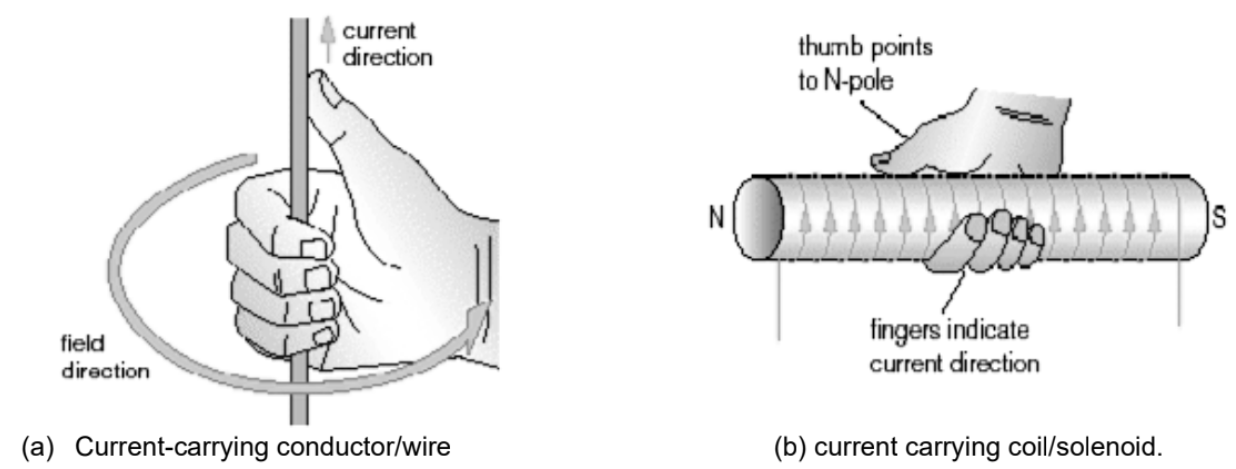
\includegraphics[width=.8\textwidth]{assets/rhgr.png}
	\caption{Right-hand grip rule}
	\label{fig:rhgr}
\end{figure}

Typical field lines (\cref{fig:bfield-lines}):
\begin{figure}[htpb]
	\centering
	\begin{minipage}{.65\textwidth}
		\centering
		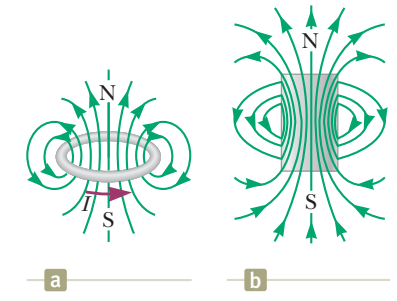
\includegraphics[width=.7\textwidth]{assets/bfields-1.png}
		\caption{Field lines for (a) circular coil and (b) bar magnet}
	\end{minipage}
	\begin{minipage}{.34\textwidth}
		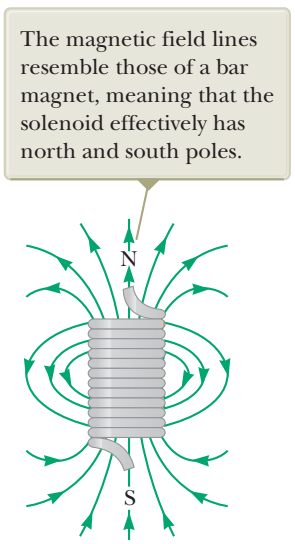
\includegraphics[width=.7\textwidth]{assets/bfields-solenoid.png}
		\caption{Field lines for solenoid}
	\end{minipage}
	\label{fig:bfield-lines}
\end{figure}
The direction of \(\va{B}\) at any point is tangent to the magnetic field line at that point.

\begin{example}{}{ferrous-core}
	For solenoids, inserting a \bf{soft iron core} magnetises the core in the same direction,
	adding to the magnetic flux density \(\implies\) strengthens net magnetic field.
\end{example}

\begin{definition}{Magnetic flux density}{bdensity}
	Force acting \it{per unit current per unit length}
	on a conductor placed perpendicular to a magnetic field [tesla: \unit{\tesla}]
	\\\\
	\footnotesize
	Magnetic flux density is \underline{1 tesla} if force per unit current per unit length
	acting on a conductor placed perpendicular to the \(\va{B}\)-field is \qty{1}{\newton\per\ampere\per\metre}.
\end{definition}

\section{FLHR}
\bf{Fleming's left-hand rule} determines the direction of the
magnetic force \(\va{F}\) from the direction of current
and magnetic field, v.v.
\begin{marginfigure}
	\centering
	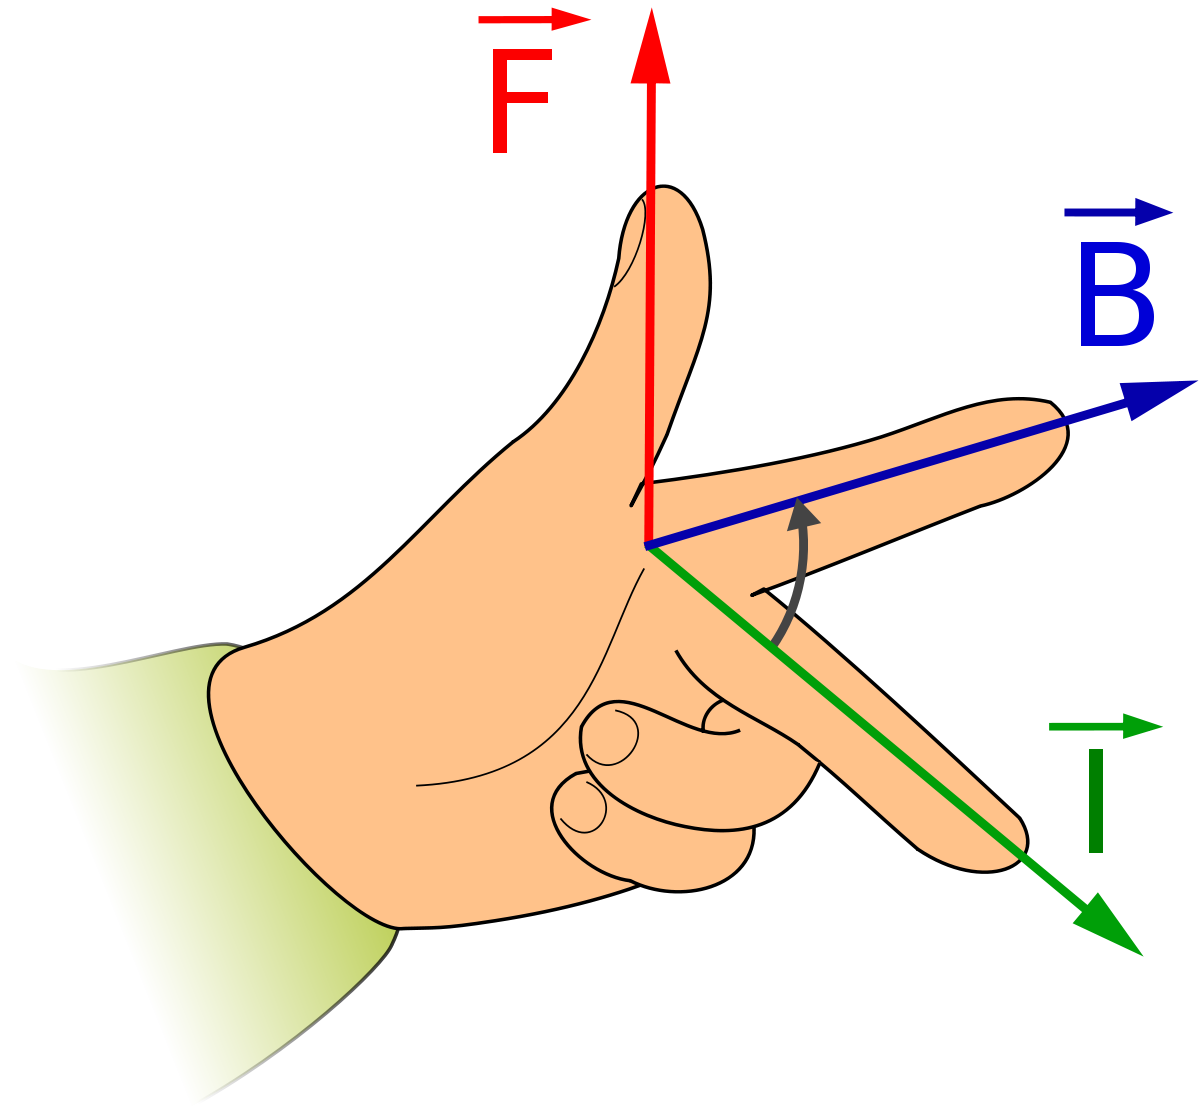
\includegraphics[width=.7\textwidth]{assets/flhr.png}
	\caption{Fleming's left-hand rule}
\end{marginfigure}

The \term{\bf{magnetic force}} acting on a straight conductor of length \(L\) carrying a current \(I\) in a magnetic field
of flux density \(B\) is
\begin{equation*}
	F_B = B_\perp IL
\end{equation*}
where \(B_\perp\) is the component of \(\va{B}\) perpendicular to the conductor.

\subsection{Like currents attract, unlike currents repel}
This is an application of FLHR. Parallel conductors carrying currents
in the \it{same direction} experience an attractive force on each other (by N3L);
currents in the \it{opposite direction} result in a repulsive force on each other (by N3L).
\begin{figure}[htpb]
	\centering
	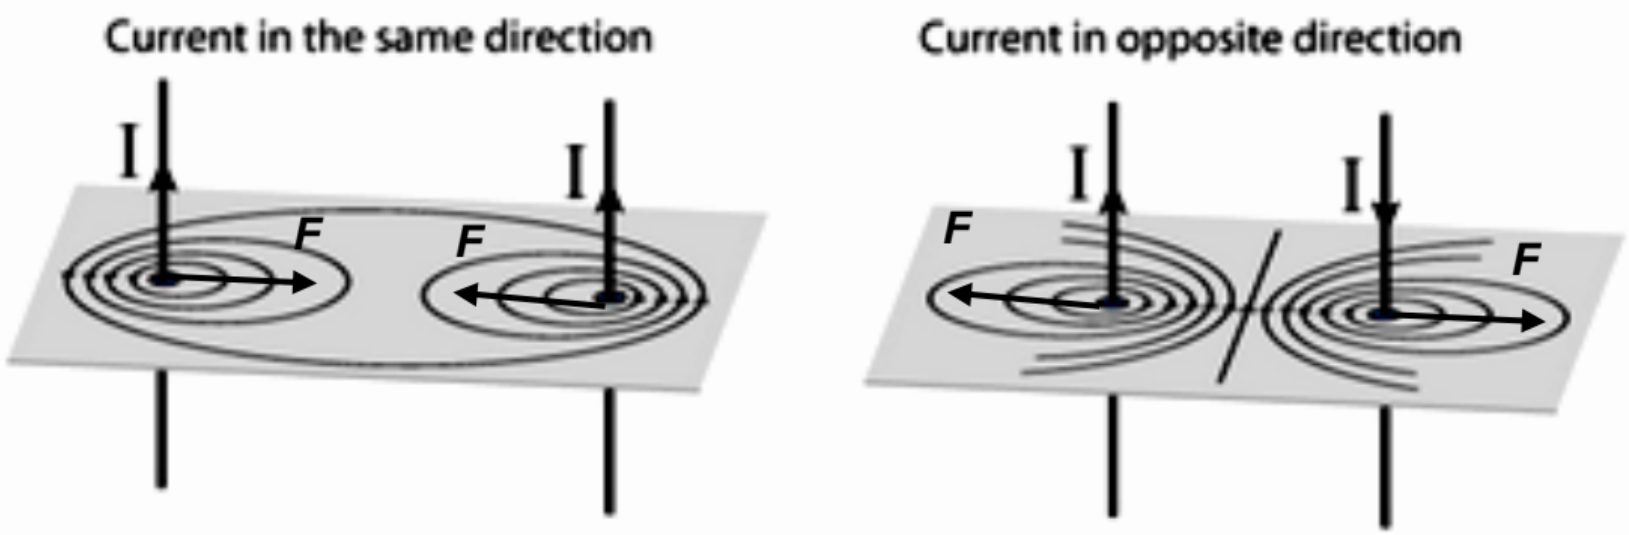
\includegraphics[width=.8\textwidth]{assets/like-unlike-currents.png}
	\caption{Like currents attract, unlike currents repel}
\end{figure}

\subsection{DC motor}
We can determine the direction of \(\va{F}\) on either side of the motor's coil
using FLHR, and hence the direction of rotation.
\begin{marginfigure}
	\centering
	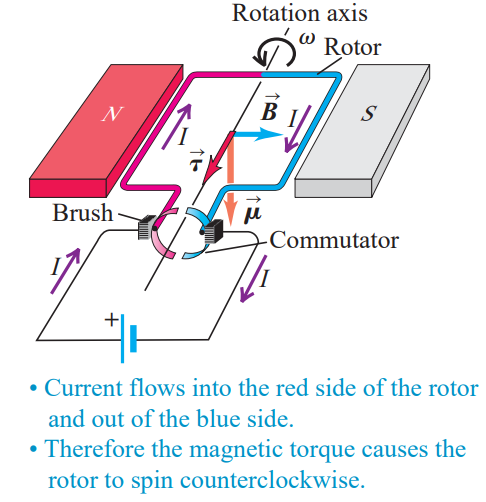
\includegraphics[width=\textwidth]{assets/dc-motor.png}
	\caption{A d.c.~motor}
\end{marginfigure}
Taking the side of the coil parallel to the current to have length \(L\),
and the side of the coil perpendicular to the current to have length \(w\), the magnetic force on each side of the coil is
\[F = nBIL\]
Since the force on the \term{pink} and \textcolor{jiyoblue}{blue} sides is equal, the coil only rotates.
With \(\theta\coloneq \) the angle between the plane of the coil and the magnetic field, the torque on the coil is
\begin{align*}
	\tau\ab(\theta) & = Fd = nBIL\cdot w\sin\theta \\
	\max\tau        & = nBILw
\end{align*}

\section{Moving charge in \(\va{B}\)-field}
\begin{marginfigure}
	\centering
	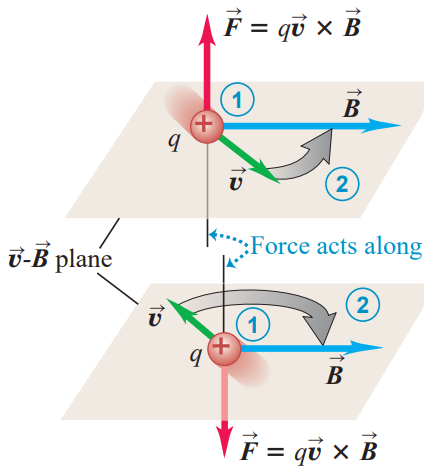
\includegraphics[width=\textwidth]{assets/flhr-moving-q.png}
	\caption{Moving positive charge in \(\va{B}\)-field}
	\label{fig:flhr-moving-q}
\end{marginfigure}
A moving charge \(q\) with velocity \(v\) experiences a magnetic force.
\[F = B_\perp q v\]
A negative charge experiences \(\va{F}\) in the opposite direction.

\begin{marginfigure}
	\centering
	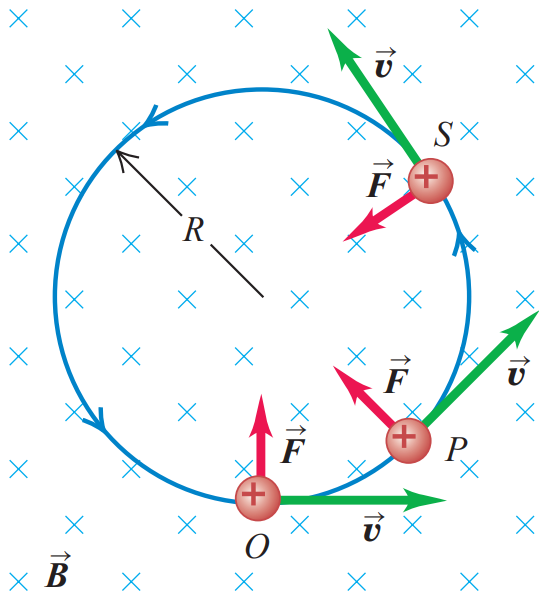
\includegraphics[width=.8\textwidth]{assets/q-circle.png}
	\caption{Moving charge in uniform \(\va{B}\)-field}
	\label{fig:moving-q-circular}
\end{marginfigure}
In a \it{uniform} magnetic field, the magnetic force provides
the charge with centripetal acceleration.
\begin{example}{}{why-constant-v}
	\it{Why does the charge move with constant speed?}

	Magnetic force \(\va{F}\) and the velocity of the charge \(\va{v}\) are always
	perpendicular to each other. Since the magnitudes of \(B\) and \(q\)
	are constant, magnitude of \(v\) is also constant.
\end{example}
\begin{align*}
	Bqv & = \f{mv^2}{r} \\
	r   & = \f{mv}{Bq}
\end{align*}
The charge will continue to trace a circle \it{only} if
the charge enters perpendicular to the field \(\va{v} \perp \va{B}\).

Otherwise, only the perpendicular component of \(\va{v}\), \(v_\perp\), contributes to the magnetic force.
\(v_\parallel\) remains constant, causing the charge to trace a helix.
For a magnetic field \(\va{B} = B\ii\), and a velocity \(\va{v} = v\cos\theta\ii + v\sin\theta\jj\), the radius of the helix is
\begin{align*}
	Bqv_\perp & = \f{m{v_\perp}^2}{r}                       \\
	r         & = \f{mv\sin\theta}{Bq}                      \\
	T         & = \f{2\pi r}{v_\perp} = \f{2\pi m}{Bq}      \\
	p         & = v_\parallel T = \f{2\pi mv\cos\theta}{Bq}
\end{align*}

\subsection{Velocity selector}
\begin{marginfigure}
	\centering
	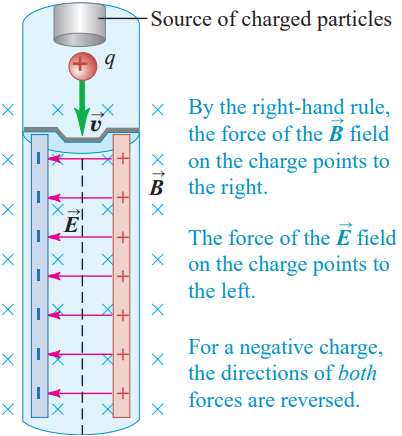
\includegraphics[width=.8\textwidth]{assets/v-selector.png}
	\caption{Velocity selector}
	\label{fig:v-selector}
\end{marginfigure}

Coinciding an \(\va{E}\) field with a \(\va{B}\) field creates a
\term{velocity selector}. For the particle's path to remain undeflected,
\(\va{F}_E = -\va{F}_B\), so
\begin{align*}
	qE & = Bqv      \\
	v  & = \f{E}{B}
\end{align*}
